% Binomial(n, 3/n) for n = 6 and n = 30 against the Poisson law of parameter 3 (dots). Generated by a short script.
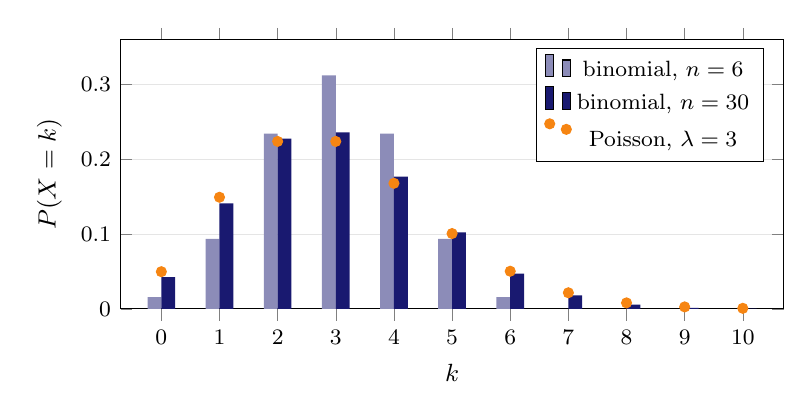
\begin{tikzpicture}
\begin{axis}[width=10cm,height=5cm,ybar=0pt,bar width=5pt,xmin=-0.7,xmax=10.7,ymin=0,ymax=0.36,xtick={0,...,10},xlabel={$k$},ylabel={$P(X=k)$},
  tick label style={font=\footnotesize},label style={font=\small},legend style={font=\footnotesize},legend pos=north east,ymajorgrids,grid style={black!10}]
\addplot[fill=MidnightBlue!50,draw=none] coordinates {(0,0.01562) (1,0.09375) (2,0.23438) (3,0.31250) (4,0.23438) (5,0.09375) (6,0.01562)};
\addlegendentry{binomial, $n=6$}
\addplot[fill=MidnightBlue,draw=none] coordinates {(0,0.04239) (1,0.14130) (2,0.22766) (3,0.23609) (4,0.17707) (5,0.10230) (6,0.04736) (7,0.01804) (8,0.00576) (9,0.00157) (10,0.00037)};
\addlegendentry{binomial, $n=30$}
\addplot[only marks,mark=*,mark size=1.8pt,BurntOrange] coordinates {(0,0.04979) (1,0.14936) (2,0.22404) (3,0.22404) (4,0.16803) (5,0.10082) (6,0.05041) (7,0.02160) (8,0.00810) (9,0.00270) (10,0.00081)};
\addlegendentry{Poisson, $\lambda=3$}
\end{axis}
\end{tikzpicture}
